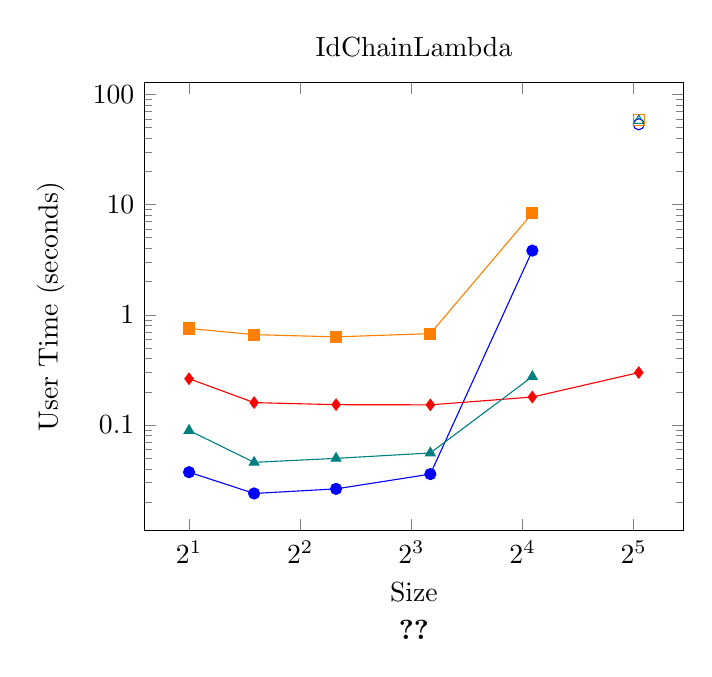
\begin{tikzpicture}
\begin{axis}
[title=IdChainLambda,
xlabel={Size},
ylabel={User Time (seconds)},
legend to name=legend,
legend columns=2,
xmode=log,
log basis x={2},
ymode=log,
log basis y={10},
yticklabel={
  \pgfkeys{/pgf/fpu=true}
  \pgfmathparse{pow(10,\tick)}
  \pgfmathprintnumber[fixed relative,precision=3]{\pgfmathresult}
  \pgfkeys{/pgf/fpu=false}
}]
\addplot [
color=blue,
mark=o,
only marks,
forget plot
] coordinates {
(33.0,53.595605) 
};
\addplot [
color=orange,
mark=square,
only marks,
forget plot
] coordinates {
(33.0,58.7287) 
};
\addplot [
color=red,
mark=diamond,
only marks,
forget plot
] coordinates {

};
\addplot [
color=teal,
mark=triangle,
only marks,
forget plot
] coordinates {
(33.0,57.836192) 
};
\addplot [
color=blue,
mark=*
] coordinates {
(17.0,3.825269) 
(9.0,3.5874e-2) 
(5.0,2.6344e-2) 
(3.0,2.3944e-2) 
(2.0,3.7351e-2) 
};
\addlegendentry{Agda}
\addplot [
color=orange,
mark=square*
] coordinates {
(17.0,8.356067) 
(9.0,0.675194) 
(5.0,0.630907) 
(3.0,0.661018) 
(2.0,0.752452) 
};
\addlegendentry{Idris 2}
\addplot [
color=red,
mark=diamond*
] coordinates {
(33.0,0.299094) 
(17.0,0.179468) 
(9.0,0.15249) 
(5.0,0.152985) 
(3.0,0.159782) 
(2.0,0.263118) 
};
\addlegendentry{Lean 4}
\addplot [
color=teal,
mark=triangle*
] coordinates {
(17.0,0.275027) 
(9.0,5.5781e-2) 
(5.0,4.9849e-2) 
(3.0,4.5868e-2) 
(2.0,8.9283e-2) 
};
\addlegendentry{Rocq}
\end{axis}
\node[anchor=north] at (current axis.below south) {\ref{legend}};
\end{tikzpicture}
